\chapter{Théories des vitesses de réaction}\label{ch:b3:rate-theories}

En 2017 fut autorisé un médicament qui ne diffère d'un médicament plus
ancien que par un détail~: les six atomes d'hydrogène de ses deux
groupes méthoxy sont des atomes de deutérium. Le foie dégrade le
principe actif en coupant précisément ces liaisons C--H, et une liaison
C--D se coupe plusieurs fois plus lentement~: la molécule lourde reste
plus longtemps dans le sang, et se prend à doses plus faibles et moins
fréquentes. Rien dans la loi d'Arrhenius n'explique pourquoi un neutron
dans un noyau ralentirait une réaction. Ce chapitre établit les
constantes de vitesse à partir des propriétés moléculaires~: d'abord à
partir des collisions, puis à partir de la forme de la \omterm{def:b3:computational-chemistry:pes}{surface d'énergie
potentielle} et des fonctions de partition de la \omterm{def:b3:rate-theories:tst}{théorie de l'état de
transition}, qui prévoit l'ampleur de tels effets isotopiques~; il se
termine par les réactions en solution, où le solvant impose une limite
de vitesse.

\begin{recall}
Le volume de première année a défini la constante de vitesse, la loi
d'Arrhenius $k =
A\eu^{-E_a/RT}$ avec son énergie d'activation et son facteur
préexponentiel, les actes élémentaires, l'état de transition, le profil
énergétique le long de la coordonnée réactionnelle et le postulat de
Hammond. Le volume de deuxième année a défini la force ionique et les
coefficients d'activité, avec la loi limite de Debye--Hückel
$\log\gamma_i = -Az_i^2\sqrt I$ ($A \approx
0.51$ dans l'eau à \qty{25}{\celsius}), et a ajusté des droites par les
moindres carrés. Le
\Cref{ch:b3:computational-chemistry} a introduit les \omterm{def:b3:computational-chemistry:pes}{surfaces d'énergie
potentielle}~; les
\cref{ch:b3:partition-functions,ch:b3:statistical-thermo-applied} ont
calculé des constantes d'équilibre à partir des fonctions de partition
et des \omterm{def:b3:quantum-model-systems:oscillator}{énergies de point zéro}. De la physique~: la distribution des
vitesses moléculaires de Maxwell--Boltzmann, et la loi de Fick de la
diffusion.
\end{recall}

\begin{omfigure}
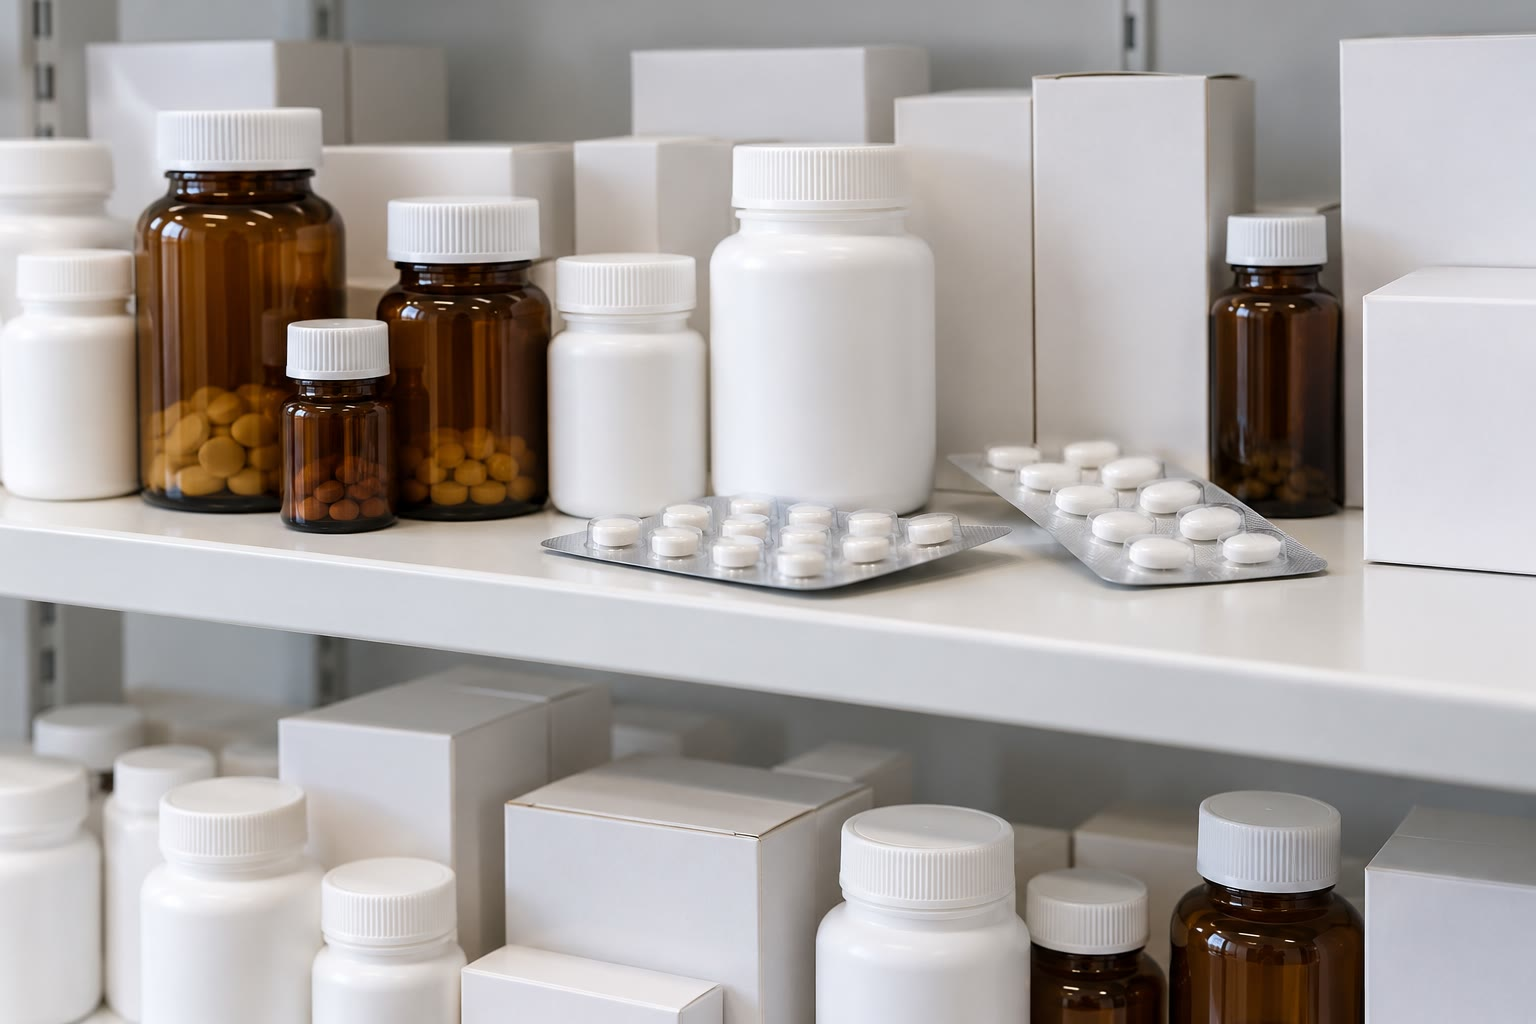
\includegraphics[width=0.6\linewidth]{images/book4/ai/b3-12-pharmacy.jpg}

{\small Des médicaments sur l'étagère d'une pharmacie. Remplacer
l'hydrogène par du deutérium sur les liaisons que le foie attaque en
premier peut allonger la durée de séjour d'un médicament dans
l'organisme.}
\end{omfigure}

\section{La théorie des collisions}

Deux molécules d'un gaz ne peuvent réagir que si elles se rencontrent.
Modélisons-les par des sphères dures de diamètres $d_{\mathrm A}$ et
$d_{\mathrm B}$~: elles entrent en collision quand leurs centres passent
à moins de $d =
\frac12(d_{\mathrm A} + d_{\mathrm B})$ l'un de l'autre.

\begin{definition}[Section efficace de collision, facteur stérique]\label{def:b3:rate-theories:collision}
La \emph{section efficace de collision}\index{section efficace de collision} de deux molécules
est l'aire $\sigma = \pi d^2$ du disque, perpendiculaire à leur vitesse
relative, à l'intérieur duquel doit passer le centre de l'une pour
qu'elle heurte l'autre. Le
\emph{facteur stérique}\index{facteur sterique@facteur stérique} $P$ est
le rapport entre le facteur préexponentiel mesuré d'une réaction et celui
que prévoit la théorie des collisions.
\end{definition}

\begin{omfigure}
\begin{tikzpicture}[font=\small, >=Stealth]
  \shade[ball color=omDef!40] (0,0) circle (0.45);
  \node at (0,0) {A};
  \draw[black!50, dashed] (-0.0,0.85) -- (5.2,0.85) (-0.0,-0.85) -- (5.2,-0.85);
  \draw[black!60] (0,0) ellipse (0.25 and 0.85);
  \draw[<->] (-0.45,0) -- (-0.45,0.85) node[midway, left] {$d$};
  \shade[ball color=omThm!40] (3.3,0.55) circle (0.4);
  \node at (3.3,0.55) {B};
  \shade[ball color=omThm!20] (4.6,1.45) circle (0.4);
  \node at (4.6,1.45) {B};
  \draw[->, thick] (0.6,0) -- (2.2,0) node[midway, below] {$v_{\mathrm{rel}}\,\Delta t$};
  \node[anchor=west, align=left, font=\scriptsize] at (5.3,0) {cylindre de\\ section\\ $\sigma = \pi d^2$};
  \node[font=\scriptsize, anchor=south] at (3.3,1.0) {touchée};
  \node[font=\scriptsize, anchor=south] at (4.6,1.9) {manquée};
\end{tikzpicture}

{\small Le cylindre de collision. Animée de la vitesse relative
$v_{\mathrm{rel}}$, la molécule A balaie
pendant une durée $\Delta t$ un cylindre de section $\sigma = \pi d^2$,
où $d$ est la somme des deux rayons~; toute molécule B dont le centre
s'y trouve est heurtée.}
\end{omfigure}

\begin{theorem}[Constante de vitesse de la théorie des collisions]\label{thm:b3:rate-theories:collision}
Si toute collision dont l'énergie cinétique selon la ligne des centres
dépasse un seuil $E_0$ (par mole) conduit à la réaction, la constante de
vitesse de $\mathrm{A + B} \to$
produits vaut
\[
  k = \sigma\bar v_{\mathrm{rel}}N_A\,\eu^{-E_0/RT}, \qquad \bar v_{\mathrm{rel}} = \sqrt{\frac{8kT}{\pi\mu}},\
  \mu = \frac{m_{\mathrm A}m_{\mathrm B}}{m_{\mathrm A} + m_{\mathrm B}} .
\]
\end{theorem}

\begin{proof}[Démonstration partielle]
Pendant une durée $\Delta t$, une molécule A balaie un volume
$\sigma v_{\mathrm{rel}}\Delta t$ et heurte les
$n_{\mathrm B}\sigma v_{\mathrm{rel}}\Delta t$ molécules B qu'il
contient~: la fréquence des collisions par unité de volume
vaut $\sigma\bar v_{\mathrm{rel}}n_{\mathrm A}n_{\mathrm B}$, où
$\bar v_{\mathrm{rel}}$ est la vitesse relative moyenne donnée par la
distribution de Maxwell--Boltzmann (admise de la physique, avec la \omterm{def:b3:quantum-model-systems:oscillator}{masse
réduite}). Pondérer chaque collision par sa vitesse et ne garder que
celles dont l'énergie selon la ligne des centres dépasse le seuil laisse
la fraction
$\eu^{-E_0/RT}$ de la fréquence des collisions (l'intégration sur le
paramètre d'impact est admise). Passer des densités en nombre aux
concentrations molaires multiplie par
$N_A$.
\end{proof}

Comme $\bar v_{\mathrm{rel}} \propto \sqrt T$, l'énergie d'activation
$E_a = RT^2\,\dd\ln k/\dd T$ vaut $E_0 + \frac12RT$,
voisine du seuil. Le facteur préexponentiel est de l'ordre de
$10^{11}$~\unit{L.mol^{-1}.s^{-1}} pour de petites molécules. Les
facteurs mesurés sont souvent bien plus petits~: $P \ll 1$ pour des
molécules qui doivent se rencontrer dans une orientation particulière,
et la section efficace n'a pas de valeur unique pour les molécules
réelles, qui ne sont pas des sphères dures. La théorie des collisions
donne l'ordre de grandeur et la dépendance en température~; elle ne peut
pas donner $E_0$, qui exige la \omterm{def:b3:computational-chemistry:pes}{surface d'énergie potentielle}.

\section{Surfaces d'énergie potentielle}

La réaction $\mathrm{H_A + H_BH_C \to H_AH_B + H_C}$ est la plus simple
qui soit. Pour une approche colinéaire, l'énergie dépend de deux
distances, $r_{\mathrm{AB}}$ et $r_{\mathrm{BC}}$, et peut se représenter
par une carte.

\begin{definition}[Point selle, chemin d'énergie minimale]\label{def:b3:rate-theories:saddle}
Un \emph{point selle}\index{point selle} (ou point col) d'une \omterm{def:b3:computational-chemistry:pes}{surface
d'énergie potentielle} est un point où le gradient s'annule, l'énergie
étant maximale dans une direction et minimale dans toutes les autres. Le
\emph{chemin d'énergie minimale}\index{chemin d'energie minimale@chemin d'énergie minimale}
est le chemin de plus grande pente qui descend du point selle vers les
vallées des réactifs et des produits~; sa longueur mesurée le long du
chemin est la coordonnée réactionnelle, et le point selle est l'état de
transition.
\end{definition}

\begin{omfigure}
\begin{tikzpicture}
\begin{axis}[ompes, width=0.62\linewidth, xmin=0.4, xmax=3.0, ymin=0.4, ymax=3.0,
  xlabel={$r_{\mathrm{AB}}$ / \AA}, ylabel={$r_{\mathrm{BC}}$ / \AA},
  colorbar, colorbar style={ylabel={$E$ / eV}, ylabel style={font=\small},
  yticklabel style={font=\small}}, point meta min=-4.7, point meta max=-0.8]
\addplot3[contour prepared={labels=false}, thick] table {figdata/out/bachelor-3-pes-collinear-contours.dat};
\addplot3[ompath] table[x=x, y=y, z expr=0] {figdata/out/bachelor-3-pes-collinear-mep.dat};
\node[omsaddle] at (axis cs:0.918,0.918,0) {};
\node[font=\small, anchor=south west] at (axis cs:0.95,0.95,0) {point selle};
\node[font=\small, anchor=west, fill=white, fill opacity=0.85, text opacity=1, inner sep=1.5pt] at (axis cs:2.05,1.0,0) {$\mathrm{H_A + H_BH_C}$};
\node[font=\small, anchor=west, fill=white, fill opacity=0.85, text opacity=1, inner sep=1.5pt] at (axis cs:0.95,2.55,0) {$\mathrm{H_AH_B + H_C}$};
\node[font=\small, anchor=north east] at (axis cs:2.95,2.95,0) {$\ce{H + H + H}$};
\end{axis}
\end{tikzpicture}

{\small Une \omterm{def:b3:computational-chemistry:pes}{surface d'énergie potentielle} modèle pour $\ce{H + H2}$
colinéaire (forme LEPS construite à partir de la courbe de Morse de
\ce{H2}, avec un paramètre de Sato de 0.17 choisi comme constante
modèle). Courbes de niveau de \qty{-4.65}{eV} à \qty{-0.8}{eV}, zéro
d'énergie pour trois atomes séparés~;
les vallées se situent à \qty{-4.75}{eV}, la profondeur du puits de
\ce{H2}. En tirets~: le \omterm{def:b3:rate-theories:saddle}{chemin d'énergie minimale}, qui franchit le \omterm{def:b3:rate-theories:saddle}{point
selle} symétrique en $r_{\mathrm{AB}} = r_{\mathrm{BC}} = \qty{0.92}{\angstrom}$,
\qty{0.27}{eV} au-dessus des vallées dans ce modèle.}
\end{omfigure}

Le chemin sort de la vallée des réactifs, où $r_{\mathrm{BC}}$ reste
voisine de la longueur de liaison de \ce{H2} pendant que A s'approche,
franchit le \omterm{def:b3:rate-theories:saddle}{point selle}, et descend dans la vallée des produits. Au \omterm{def:b3:rate-theories:saddle}{point
selle}, les deux liaisons sont étirées à \qty{0.92}{\angstrom}~:
l'ancienne liaison est à moitié rompue et la nouvelle à moitié formée,
et le coût énergétique de ce compromis est la barrière. Pour la réaction
symétrique, le \omterm{def:b3:rate-theories:saddle}{point selle} se trouve sur la diagonale~; pour une
réaction exothermique, il se déplace vers la vallée des réactifs (une
barrière précoce, un état de transition proche des réactifs, comme le dit
le postulat de Hammond), pour une réaction endothermique vers la vallée
des produits (une barrière tardive). Sa position décide de l'énergie qui
aide~: l'énergie de translation, dirigée le long de la vallée d'entrée,
fait passer les molécules au-dessus d'une barrière précoce~; une
barrière tardive, située après un coude, se franchit plus facilement
avec de l'énergie de vibration dans la liaison qui se rompt. Ce sont les
règles de Polanyi, confirmées par des expériences en jets moléculaires.

\section{La théorie de l'état de transition}

\begin{definition}[Complexe activé]\label{def:b3:rate-theories:activated-complex}
Le \emph{complexe activé}\index{complexe active@complexe activé} d'un
acte élémentaire est l'ensemble des configurations du système réactif
situées dans une mince tranche autour du \omterm{def:b3:rate-theories:saddle}{point selle}, perpendiculaire au
\omterm{def:b3:rate-theories:saddle}{chemin d'énergie minimale}~; on le traite comme une espèce
$\ce{AB^{\ddagger}}$, dotée de sa propre fonction de partition.
\end{definition}

\begin{definition}[Théorie de l'état de transition, coefficient de transmission]\label{def:b3:rate-theories:tst}
La \emph{théorie de l'état de transition}\index{theorie de l'etat de transition@théorie de l'état de transition} suppose
que les \omterm{def:b3:rate-theories:activated-complex}{complexes activés} sont en équilibre avec les réactifs, que tout
complexe qui traverse la région du \omterm{def:b3:rate-theories:saddle}{point selle} vers les produits
continue jusqu'à les former, et que le mouvement selon la coordonnée
réactionnelle est une translation libre. Le
\emph{coefficient de transmission}\index{coefficient de transmission} $\kappa \le 1$
corrige pour les complexes qui retraversent vers les réactifs.
\end{definition}

\begin{theorem}[Équation d'Eyring]\label{thm:b3:rate-theories:eyring}
Pour un acte élémentaire $\mathrm{A + B} \to \mathrm{AB}^{\ddagger} \to$ produits,
\[
  k = \kappa\frac{k_BT}{h}\overline{K}{}^{\ddagger}, \qquad
  \overline{K}{}^{\ddagger} = \frac{\bar q^{\ddagger}/N_A}{(q_{\mathrm A}/N_A)(q_{\mathrm B}/N_A)}\,\eu^{-\Delta E_0^{\ddagger}/RT},
\]
où $\bar q^{\ddagger}$ est la fonction de partition du \omterm{def:b3:rate-theories:activated-complex}{complexe activé}
privée du mouvement selon la coordonnée réactionnelle, les $q$ sont des
fonctions de partition molaires par unité de volume, et
$\Delta E_0^{\ddagger}$ est la hauteur du niveau de point zéro du
complexe au-dessus de celui des réactifs. Sous forme thermodynamique,
avec $c^\circ = \qty{1}{mol/L}$ et la
molécularité $m$,
\[
  k = \kappa\frac{k_BT}{h}(c^\circ)^{1-m}\,\eu^{\Delta^{\ddagger}S^\circ/R}\,\eu^{-\Delta^{\ddagger}H^\circ/RT}.
\]
C'est l'\emph{équation d'Eyring}\index{equation d'Eyring@équation d'Eyring}~; $k_B$ est la
constante de Boltzmann, notée ainsi pour éviter la confusion avec $k$.
\end{theorem}

\begin{proof}
Quasi-équilibre~: $[\ce{AB^{\ddagger}}] = K^{\ddagger}[\mathrm A][\mathrm B]$,
$K^{\ddagger}$ étant tiré des fonctions de partition
(\cref{thm:b3:statistical-thermo-applied:k-from-q}, écrit avec des
concentrations).
Parmi les vibrations du complexe, l'une est le mouvement selon la
coordonnée réactionnelle~: une vibration très lâche de fréquence
$\nu \ll k_BT/h$, dont la fonction de partition
vaut $k_BT/h\nu$ (limite de haute température de la
\cref{prop:b3:partition-functions:q-vib})~; donc $q^{\ddagger} = \bar q^{\ddagger}k_BT/h\nu$.
Les complexes passent vers les produits à la fréquence $\nu$ de ce
mouvement, si bien que la vitesse vaut
$\nu[\ce{AB^{\ddagger}}] = \nu\frac{k_BT}{h\nu}\overline{K}{}^{\ddagger}[\mathrm A][\mathrm B]$~:
la fréquence inconnue $\nu$ se simplifie. En écrivant
$\overline{K}{}^{\ddagger} = (c^\circ)^{1-m}\eu^{-\Delta^{\ddagger}G^\circ/RT}$ et $\Delta^{\ddagger}G^\circ = \Delta^{\ddagger}H^\circ - T\Delta^{\ddagger}S^\circ$,
on obtient la seconde forme, où l'on insère $\kappa$ pour tenir compte
des retraversées.
\end{proof}

Le facteur $k_BT/h$ vaut \qty{6.2e12}{s^{-1}} à \qty{298}{K}~: c'est la
vitesse d'un acte monomoléculaire sans barrière ni perte d'entropie.
Tout ce qui est propre à la réaction réside dans les grandeurs
d'activation.

\begin{definition}[Enthalpie libre, enthalpie et entropie d'activation]\label{def:b3:rate-theories:activation}
L'\emph{enthalpie libre d'activation}\index{enthalpie libre d'activation}
$\Delta^{\ddagger}G^\circ$, l'\emph{enthalpie d'activation}\index{enthalpie d'activation} $\Delta^{\ddagger}H^\circ$ et
l'\emph{entropie d'activation}\index{entropie d'activation} $\Delta^{\ddagger}S^\circ$ d'un acte
élémentaire sont l'enthalpie libre, l'enthalpie et l'entropie standard
de formation du \omterm{def:b3:rate-theories:activated-complex}{complexe activé} (privé de son mouvement selon la
coordonnée réactionnelle) à partir des réactifs, définies par l'\omterm{thm:b3:rate-theories:eyring}{équation
d'Eyring}.
\end{definition}

\begin{proposition}[Énergie d'activation et enthalpie d'activation]\label{prop:b3:rate-theories:ea-dh}
Pour une réaction en solution, $E_a = \Delta^{\ddagger}H^\circ + RT$~;
pour une réaction bimoléculaire en phase gazeuse,
$E_a = \Delta^{\ddagger}H^\circ + 2RT$.
\end{proposition}

\begin{proof}
$E_a = RT^2\,\dd\ln k/\dd T$, et $\ln k = \ln T + \Delta^{\ddagger}S^\circ/R - \Delta^{\ddagger}H^\circ/RT + $ cste~: $E_a =
RT + \Delta^{\ddagger}H^\circ$ quand les paramètres d'activation ne
varient pas avec $T$. En solution, c'est le résultat. En phase gazeuse,
la relation de van 't Hoff pour $K^{\ddagger}$ écrite
en concentrations fait intervenir l'énergie interne,
$\Delta^{\ddagger}U^\circ = \Delta^{\ddagger}H^\circ - \Delta n^{\ddagger}RT$
avec $\Delta n^{\ddagger} = 1 - m$~: pour $m = 2$, $E_a = \Delta^{\ddagger}H^\circ + 2RT$.
\end{proof}

L'\omterm{def:b3:rate-theories:activation}{entropie d'activation} renseigne sur la structure de l'état de
transition. Deux molécules qui s'unissent en un seul complexe perdent de
la liberté de translation et de rotation~: $\Delta^{\ddagger}S^\circ$ est
fortement négative, de $-50$ à $-150$ \unit{J.K^{-1}.mol^{-1}}, pour les
actes associatifs et les états de transition cycliques. Une molécule qui
relâche une liaison en route vers sa dissociation gagne de la liberté~:
$\Delta^{\ddagger}S^\circ > 0$.

\begin{proposition}[Écarts-types d'une droite ajustée]\label{prop:b3:rate-theories:slope-uncertainty}
Pour une droite des moindres carrés $y = a + bx$ passant par $n$ points
dont les $y$ sont entachés d'erreurs indépendantes de même variance,
estimée par $s^2 = \sum_i(y_i - a - bx_i)^2/(n - 2)$,
la pente et l'ordonnée à l'origine ont pour écarts-types
\[
  s_b = \frac{s}{\sqrt{\sum_i(x_i - \bar x)^2}}, \qquad
  s_a = s\sqrt{\frac1n + \frac{\bar x^2}{\sum_i(x_i - \bar x)^2}} .
\]
\end{proposition}

\begin{proof}
$b = \sum_i(x_i - \bar x)y_i/S_{xx}$, avec $S_{xx} = \sum_i(x_i - \bar x)^2$, est une combinaison linéaire de
$y_i$ indépendants de variance $\sigma^2$~: sa variance vaut $\sigma^2\sum_i(x_i - \bar x)^2/S_{xx}^2 = \sigma^2/S_{xx}$.
De même, $a = \bar y - b\bar x$, et $\bar y$ et $b$ ne sont pas corrélés
(leur covariance vaut
$\sigma^2\sum_i(x_i - \bar x)/(nS_{xx}) = 0$), donc $\operatorname{var}a = \sigma^2/n + \bar x^2\sigma^2/S_{xx}$.
Remplacer $\sigma^2$
par son estimation $s^2$ (le diviseur $n - 2$ tient compte des deux
paramètres ajustés, ce qui est admis) donne le résultat.
\end{proof}

\begin{method}[Un tracé d'Eyring avec ses incertitudes]\label{met:b3:rate-theories:eyring-plot}
\begin{enumerate}
  \item Mesurer $k$ à cinq températures ou plus, réparties sur 30 à
        \qty{40}{K}.
  \item Tracer $y = \ln(k/T)$ en fonction de $x = 1/T$ et ajuster la
        droite des moindres carrés $y = a + bx$.
  \item $\Delta^{\ddagger}H^\circ = -Rb$ et $\Delta^{\ddagger}S^\circ = R[a - \ln(k_B/h)]$ ($\ln(k_B/h) = 23.760$ avec $k$ en
        \unit{s^{-1}}).
  \item Leurs écarts-types sont $Rs_b$ et $Rs_a$~; un intervalle de
        confiance à 95\,\% s'obtient en les multipliant par le $t$ de
        Student à $n - 2$ degrés de liberté (3.18 pour
        cinq points).
  \item L'ordonnée à l'origine se situe loin du domaine mesuré, en
        $1/T = 0$~: $\Delta^{\ddagger}S^\circ$
        est toujours bien moins précise que $\Delta^{\ddagger}H^\circ$, et
        les deux erreurs sont corrélées.
\end{enumerate}
\end{method}

\begin{omfigure}
\begin{tikzpicture}
\begin{axis}[width=0.74\linewidth, height=6.2cm, xmin=3.12, xmax=3.62, ymin=-12.8, ymax=-6.4,
  axis lines=left, xlabel={$1000\,\mathrm K/T$}, ylabel={$\ln\bigl(k/(\mathrm s^{-1}\,\mathrm K^{-1})\bigr)$},
  tick label style={font=\small}, label style={font=\small},
  legend style={font=\scriptsize, draw=none, fill=white, fill opacity=0.85, text opacity=1,
  at={(0.98,0.98)}, anchor=north east}, legend cell align=left]
\addplot[omDef, thick] table[x=invT, y=fit] {figdata/out/bachelor-3-eyring-band-H.dat};
\addplot[omThm, thick] table[x=invT, y=fit] {figdata/out/bachelor-3-eyring-band-D.dat};
\addplot[omDef, thin, dashed, forget plot] table[x=invT, y=lo] {figdata/out/bachelor-3-eyring-band-H.dat};
\addplot[omDef, thin, dashed, forget plot] table[x=invT, y=hi] {figdata/out/bachelor-3-eyring-band-H.dat};
\addplot[omThm, thin, dashed, forget plot] table[x=invT, y=lo] {figdata/out/bachelor-3-eyring-band-D.dat};
\addplot[omThm, thin, dashed, forget plot] table[x=invT, y=hi] {figdata/out/bachelor-3-eyring-band-D.dat};
\addplot[only marks, mark=*, mark size=1.8pt, omDef, forget plot] table[x=invT, y=lnkT_H] {figdata/out/bachelor-3-eyring-points.dat};
\addplot[only marks, mark=square*, mark size=1.7pt, omThm, forget plot] table[x=invT, y=lnkT_D] {figdata/out/bachelor-3-eyring-points.dat};
\legend{médicament \ce{OCH3}, médicament \ce{OCD3}}
\end{axis}
\end{tikzpicture}

{\small Tracés d'Eyring des constantes de vitesse du problème du
week-end (données du problème) pour le médicament et son analogue
deutéré, avec les droites des moindres carrés et leurs bandes de
confiance à 95\,\% (en tirets, à peine plus larges que les droites~: les
points se dispersent d'environ 1\,\%). Les droites sont parallèles aux
incertitudes près~: même \omterm{def:b3:rate-theories:activation}{entropie d'activation}, \omterm{def:b3:rate-theories:activation}{enthalpies d'activation}
différant d'environ \qty{5}{kJ/mol}.}
\end{omfigure}

\section{Effets isotopiques cinétiques}

\begin{definition}[Effets isotopiques cinétiques]\label{def:b3:rate-theories:kie}
L'\emph{effet isotopique cinétique}\index{effet isotopique cinetique@effet isotopique cinétique} d'un acte est le
rapport $k_{\mathrm{light}}/k_{\mathrm{heavy}}$ de ses constantes de
vitesse pour deux \omterm{def:b3:rovibrational-spectroscopy:rotational-constant}{isotopologues}, le plus souvent
$k_{\mathrm H}/k_{\mathrm D}$. C'est un \emph{effet isotopique cinétique
primaire}\index{effet isotopique cinetique primaire@effet isotopique cinétique primaire}
quand la liaison à l'atome substitué se forme ou se rompt dans l'acte,
un \emph{effet isotopique cinétique secondaire}\index{effet isotopique cinetique secondaire@effet isotopique cinétique secondaire}
dans le cas contraire.
\end{definition}

\begin{proposition}[Effet isotopique cinétique primaire maximal]\label{prop:b3:rate-theories:primary-kie}
Si la vibration d'élongation d'une liaison X--H devient la coordonnée
réactionnelle, si bien que son \omterm{def:b3:quantum-model-systems:oscillator}{énergie de point zéro} est perdue dans
l'état de transition tandis que toutes les autres contributions sont
les mêmes pour H et pour D,
\[
  \frac{k_{\mathrm H}}{k_{\mathrm D}} = \exp\Bigl[\frac{hc(\tilde\nu_{\mathrm{XH}} - \tilde\nu_{\mathrm{XD}})}{2k_BT}\Bigr],
  \qquad \frac{\tilde\nu_{\mathrm{XH}}}{\tilde\nu_{\mathrm{XD}}} = \sqrt{\frac{\mu_{\mathrm{XD}}}{\mu_{\mathrm{XH}}}} .
\]
\end{proposition}

\begin{proof}
La \omterm{def:b3:computational-chemistry:pes}{surface d'énergie potentielle} est la même pour les deux \omterm{def:b3:rovibrational-spectroscopy:rotational-constant}{isotopologues}
(les électrons ne voient pas le neutron). Dans le réactif, l'élongation
X--H détient
$\frac12hc\tilde\nu_{\mathrm{XH}}$ d'\omterm{def:b3:quantum-model-systems:oscillator}{énergie de point zéro}~; dans l'état
de transition, ce mode est devenu la coordonnée réactionnelle et n'en
détient aucune. La barrière mesurée entre niveaux de point zéro est donc
plus basse pour H de $\frac12hc\tilde\nu_{\mathrm{XH}}$ et pour D de $\frac12hc\tilde\nu_{\mathrm{XD}}$~: $\Delta E_0^{\ddagger}(\mathrm D) -
\Delta E_0^{\ddagger}(\mathrm H) = \frac12hc(\tilde\nu_{\mathrm{XH}} - \tilde\nu_{\mathrm{XD}})$,
et l'\omterm{thm:b3:rate-theories:eyring}{équation d'Eyring} donne le rapport quand les autres facteurs se
compensent. Le nombre d'onde d'une élongation est proportionnel à
$1/\sqrt\mu$ (\cref{ch:b3:rovibrational-spectroscopy}).
\end{proof}

\begin{omfigure}
\begin{tikzpicture}[font=\small, >=Stealth, x=1cm, y=1cm]
  \draw[->] (-1.4,0) -- (-1.4,4.7) node[anchor=south] {$E$};
  \draw[->] (-1.4,0) -- (10.6,0) node[anchor=north east] {coordonnée réactionnelle};
  \draw[very thick, black!70] plot[smooth, tension=0.6] coordinates {(1.6,3.4) (2.1,1.6) (2.7,0.8)
    (3.3,0.6) (3.9,0.8) (4.7,2.0) (5.5,3.6) (6.2,4.0) (6.9,3.6) (7.7,2.2) (8.5,1.2) (9.2,1.0)
    (9.9,1.2) (10.4,1.7)};
  \draw[black!50, dashed] (2.8,0.6) -- (3.8,0.6);
  \draw[omDef, thick] (2.42,1.35) -- (4.2,1.35);
  \draw[omThm, thick] (2.5,1.05) -- (4.05,1.05);
  \node[omDef, font=\scriptsize, anchor=south] at (3.3,1.37) {C--H};
  \node[omThm, font=\scriptsize, anchor=north] at (3.3,1.03) {C--D};
  \draw[black, thick] (5.7,4.0) -- (6.7,4.0);
  \draw[black!40, densely dotted] (0.0,4.0) -- (5.7,4.0);
  \draw[black!40, densely dotted] (0.7,1.35) -- (2.42,1.35) (0.0,1.05) -- (2.5,1.05);
  \draw[<->, omThm] (0.0,1.05) -- (0.0,4.0) node[pos=0.5, left, font=\scriptsize] {$E_0(\mathrm D)$};
  \draw[<->, omDef] (0.7,1.35) -- (0.7,4.0) node[pos=0.5, right, font=\scriptsize] {$E_0(\mathrm H)$};
  \node[anchor=south, align=center, font=\scriptsize] at (6.2,4.05) {état de transition~: l'élongation est\\ devenue la coordonnée réactionnelle};
\end{tikzpicture}

{\small Origine de l'\omterm{def:b3:rate-theories:kie}{effet isotopique cinétique primaire}. Dans le réactif,
l'élongation C--H détient plus d'\omterm{def:b3:quantum-model-systems:oscillator}{énergie de point zéro} que l'élongation
C--D (niveaux au-dessus du fond du puits, en tirets)~; dans l'état de
transition, cette vibration est devenue la coordonnée réactionnelle, et
les deux \omterm{def:b3:rovibrational-spectroscopy:rotational-constant}{isotopologues} atteignent le même sommet. La barrière est plus
grande pour D de la différence des \omterm{def:b3:quantum-model-systems:oscillator}{énergies de point zéro}.}
\end{omfigure}

\begin{omfigure}
\begin{tikzpicture}
\begin{axis}[width=0.7\linewidth, height=5.6cm, xmin=200, xmax=800, ymin=1, ymax=50,
  ymode=log, axis lines=left, xlabel={$T$ / K}, ylabel={$k_{\mathrm H}/k_{\mathrm D}$ (maximal)},
  tick label style={font=\small}, label style={font=\small}, log ticks with fixed point,
  ytick={1,2,5,10,20,50}, legend style={font=\scriptsize, draw=none, at={(0.98,0.98)},
  anchor=north east}, legend cell align=left]
\addplot[omThm, thick] table[x=T, y=OH] {figdata/out/bachelor-3-kie.dat};
\addplot[black!60, thick] table[x=T, y=NH] {figdata/out/bachelor-3-kie.dat};
\addplot[omDef, thick] table[x=T, y=CH] {figdata/out/bachelor-3-kie.dat};
\legend{O--H (\qty{3657}{cm^{-1}}), N--H (\qty{3337}{cm^{-1}}), C--H (\qty{2917}{cm^{-1}})}
\end{axis}
\end{tikzpicture}

{\small \omterm{def:b3:rate-theories:kie}{Effet isotopique cinétique primaire} maximal en fonction de la
température, pour la perte d'une élongation C--H, N--H ou O--H
(\omterm{def:b3:rovibrational-spectroscopy:anharmonic}{transitions fondamentales} de \ce{CH4}, \ce{NH3} et \ce{H2O}~; nombres
d'onde du deutérium tirés des \omterm{def:b3:quantum-model-systems:oscillator}{masses réduites}). À \qty{298}{K}, il vaut
6.5 pour C--H~; il décroît vers 1 quand la température s'élève.}
\end{omfigure}

La valeur maximale pour C--H à température ambiante, environ 7, est une
référence. Des effets observés de 2 à 7 indiquent que la liaison C--H est
rompue dans l'étape cinétiquement déterminante~; des valeurs plus
faibles, que l'état de transition conserve une partie de l'élongation
(transferts d'hydrogène asymétriques, précoces ou tardifs), ou que l'acte
n'est pas le plus lent. Des valeurs bien supérieures à 7 à température
ambiante ne peuvent pas venir des \omterm{def:b3:quantum-model-systems:oscillator}{énergies de point zéro}~: elles révèlent
l'\omterm{def:b3:quantum-model-systems:tunnelling}{effet tunnel} (\cref{ch:b3:quantum-model-systems}), bien moins efficace
pour une particule de masse double. Les effets secondaires, dus aux
changements des vibrations de déformation des liaisons C--H voisines du
centre réactionnel, sont petits, typiquement de 0.8 à 1.2 par
deutérium~; ils distinguent, par exemple, un carbone qui devient trigonal
(sp$^3$ vers sp$^2$, $k_{\mathrm H}/k_{\mathrm D} > 1$) d'un carbone qui
devient tétraédrique ($< 1$).

\begin{method}[Mesurer un effet isotopique cinétique par compétition]\label{met:b3:rate-theories:kie}
\begin{enumerate}
  \item Effectuer la réaction sur un mélange des deux \omterm{def:b3:rovibrational-spectroscopy:rotational-constant}{isotopologues}, ou sur
        une molécule portant H sur un site et D sur un site équivalent.
  \item Arrêter à faible conversion et mesurer le rapport des produits H et
        D par spectrométrie de masse ou par RMN.
  \item Le rapport des produits, corrigé du rapport de départ, vaut
        $k_{\mathrm H}/k_{\mathrm D}$~; les deux \omterm{def:b3:rovibrational-spectroscopy:rotational-constant}{isotopologues} subissent
        exactement les mêmes conditions, ce qui rend la méthode plus
        précise que deux mesures de vitesse séparées.
\end{enumerate}
\end{method}

\section{Réactions en solution}

Dans un liquide, une molécule ne vole pas librement entre deux
collisions~: elle s'agite dans une cage de voisines, qu'elle heurte de
nombreuses fois avant de s'en échapper par diffusion. Deux réactifs qui
se rencontrent restent ensemble pendant de nombreuses collisions~: c'est
une rencontre.

\begin{definition}[Contrôle par la diffusion et par l'activation, effet de cage]\label{def:b3:rate-theories:diffusion}
Une réaction en solution est une \emph{réaction contrôlée par la
diffusion}\index{reaction controlee par la diffusion@réaction contrôlée par la diffusion}
quand la réaction est rapide à chaque rencontre, si bien que sa vitesse
est celle à laquelle les réactifs se rejoignent par diffusion~; c'est une
\emph{réaction contrôlée par l'activation}\index{reaction controlee par l'activation@réaction contrôlée par l'activation}
quand seule une petite fraction des rencontres conduit à la réaction.
L'\emph{effet de cage}\index{effet de cage} est le confinement d'une
paire de molécules par le solvant environnant, qui les fait se heurter à
plusieurs reprises au cours d'une même rencontre.
\end{definition}

\begin{proposition}[Limite de Smoluchowski]\label{prop:b3:rate-theories:smoluchowski}
La constante de vitesse d'une \omterm{def:b3:rate-theories:diffusion}{réaction contrôlée par la diffusion} entre
des sphères qui réagissent à la distance $R^*$ vaut
$k_d = 4\pi N_A(D_{\mathrm A} + D_{\mathrm B})R^*$. Avec la relation de
Stokes--Einstein
$D = k_BT/6\pi\eta a$ pour des sphères de rayon $a$ dans un solvant de
viscosité $\eta$,
et $R^* = a_{\mathrm A} + a_{\mathrm B}$ avec $a_{\mathrm A} = a_{\mathrm B}$,
\[
  k_d = \frac{8RT}{3\eta} .
\]
\end{proposition}

\begin{proof}[Démonstration partielle]
Fixons A à l'origine~; B diffuse avec le coefficient de diffusion relatif $D =
D_{\mathrm A} + D_{\mathrm B}$ et disparaît en $r = R^*$. En régime
stationnaire, le flux radial à travers toute sphère est le même,
$J = 4\pi r^2D\,\dd c/\dd r$ (loi de Fick, issue de la physique)~;
l'intégration de $R^*$, où $c = 0$, à l'infini, où $c = c_{\mathrm B}$,
donne
$J = 4\pi DR^*c_{\mathrm B}$, la vitesse par molécule A. Avec la relation
de Stokes--Einstein (admise),
$(D_{\mathrm A} + D_{\mathrm B})R^* = \frac{k_BT}{6\pi\eta}(\frac{1}{a} + \frac1a)(2a) = \frac{2k_BT}{3\pi\eta}$, et $k_d = 4\pi N_A \times
\frac{2k_BT}{3\pi\eta} = 8RT/3\eta$.
\end{proof}

\begin{example}[Limites de vitesse dans l'eau et dans l'hexane]\label{ex:b3:rate-theories:speed-limit}
% ledger: visc:H2O.25C, visc:hexane.25C
À \qty{298.15}{K}, l'eau ($\eta = \qty{0.890}{mPa.s}$) donne $k_d = 8 \times 8.314 \times
298.15/(3 \times \num{0.890e-3}) = \qty{7.4e6}{m^3.mol^{-1}.s^{-1}} = \qty{7.4e9}{L.mol^{-1}.s^{-1}}$~;
l'hexane
($\eta = \qty{0.298}{mPa.s}$), \qty{2.2e10}{L.mol^{-1}.s^{-1}}. Aucune
réaction bimoléculaire entre molécules neutres de taille ordinaire n'est
plus rapide~; les constantes mesurées voisines de ces valeurs
(désactivation d'états excités, recombinaison de radicaux) sont
contrôlées par la diffusion. Des ions de charges opposées s'attirent et
peuvent aller plus vite.
\end{example}

En solution, les ions ajoutent une contribution électrostatique à
l'activation~: l'état de transition de deux ions porte la charge
$z_{\mathrm A} + z_{\mathrm B}$, et son coefficient d'activité diffère du
produit des leurs.

\begin{definition}[Effet de sel cinétique]\label{def:b3:rate-theories:salt}
L'\emph{effet de sel cinétique}\index{effet de sel cinetique@effet de sel cinétique} est la variation de la
constante de vitesse d'une réaction entre ions avec la force ionique de
la solution.
\end{definition}

\begin{proposition}[Équation de Brønsted--Bjerrum]\label{prop:b3:rate-theories:bronsted-bjerrum}
Pour un acte entre ions de charges $z_{\mathrm A}$ et $z_{\mathrm B}$ en
solution aqueuse diluée,
\[
  \log k = \log k_0 + 2Az_{\mathrm A}z_{\mathrm B}\sqrt I,
\]
où $k_0$ est la constante de vitesse à force ionique nulle.
\end{proposition}

\begin{proof}
Dans la \omterm{def:b3:rate-theories:tst}{théorie de l'état de transition}, l'équilibre avec le \omterm{def:b3:rate-theories:activated-complex}{complexe
activé} s'écrit avec les activités~:
$[\ce{AB^{\ddagger}}] = K^{\ddagger}[\mathrm A][\mathrm B]\gamma_{\mathrm A}\gamma_{\mathrm B}/\gamma^{\ddagger}$, donc $k = k_0\gamma_{\mathrm A}\gamma_{\mathrm B}/\gamma^{\ddagger}$.
Avec la loi limite~: $\log(\gamma_{\mathrm A}\gamma_{\mathrm B}/\gamma^{\ddagger}) = -A\sqrt I[z_{\mathrm A}^2 + z_{\mathrm B}^2 - (z_{\mathrm A} + z_{\mathrm B})^2] =
2Az_{\mathrm A}z_{\mathrm B}\sqrt I$.
\end{proof}

Des ions de même signe réagissent plus vite quand on ajoute du sel
(l'atmosphère ionique écrante leur répulsion), des ions de signes opposés
plus lentement, et un réactif neutre ne présente pas d'effet de sel
primaire~: un tracé de $\log k$ en fonction de $\sqrt I$ à faible
force ionique mesure le produit des charges des espèces qui réagissent.

\begin{method}[Ce que les paramètres d'activation disent d'un mécanisme]\label{met:b3:rate-theories:mechanism-evidence}
\begin{enumerate}
  \item $\Delta^{\ddagger}S^\circ$ fortement négative~: un acte
        associatif, un état de transition ordonné ou cyclique, ou un état
        de transition qui ordonne le solvant (création de charges)~;
        positive~: un acte dissociatif.
  \item Un $k_{\mathrm H}/k_{\mathrm D}$ primaire de 2 à 7~: la liaison à
        H est rompue dans l'étape cinétiquement déterminante~; au-delà
        d'environ 10 à température ambiante~: \omterm{def:b3:quantum-model-systems:tunnelling}{effet tunnel}.
  \item La pente de $\log k$ en fonction de $\sqrt I$~: le produit
        $z_{\mathrm A}z_{\mathrm B}$ des charges qui se rencontrent dans
        l'étape cinétiquement déterminante.
  \item Une constante de vitesse voisine de $10^{10}$~\unit{L.mol^{-1}.s^{-1}}
        qui varie comme $T/\eta$~:
        contrôle par la diffusion.
\end{enumerate}
\end{method}

\begin{inthelab}[Une cuve à double enveloppe pour une étude d'Eyring]
On suit la réaction par son absorbance dans une cuve de
spectrophotomètre dont la double enveloppe est alimentée par un bain
thermostaté~; un thermocouple placé dans une cuve de référence contrôle
la température à \qty{0.1}{K} près. Cinq à sept températures, chacune
mesurée trois fois, donnent un tracé d'Eyring~; les solutions sont mises
à l'équilibre thermique dans le support avant le mélange, car une
réaction démarrée à une mauvaise température fausse les premiers points.
\end{inthelab}

\begin{history}[Eyring, Evans et Polanyi, 1935]
En 1935, Henry Eyring, à Princeton, et Meredith Gwynne Evans et Michael
Polanyi, à Manchester, publièrent indépendamment la théorie du \omterm{def:b3:rate-theories:activated-complex}{complexe
activé}. Eyring avait calculé avec Polanyi, à Berlin en 1931, la première
\omterm{def:b3:computational-chemistry:pes}{surface d'énergie potentielle} de $\ce{H + H2}$, par une méthode
semi-empirique du type de celle utilisée pour la figure de ce chapitre.
La théorie fut accueillie avec suspicion~: une revue rejeta d'abord
l'article d'Eyring comme dénué de fondement, et il ne fut publié qu'après
que d'autres physiciens s'en furent portés garants.
\end{history}

\section{Exercices}

\begin{exercise}[$\star$]\label{exo:b3:rate-theories:1}
% ledger: kin:NO+O3.A
Pour $\ce{NO + O3 -> NO2 + O2}$, on prendra $\sigma = \qty{0.43}{nm^2}$
(données de l'exercice). Calculer $\bar v_{\mathrm{rel}}$
à \qty{298}{K} ($\mu = \qty{18.46}{u}$), le facteur préexponentiel de la
théorie des collisions, et le \omterm{def:b3:rate-theories:collision}{facteur stérique}, sachant que la valeur
mesurée est $A = \qty{2.07e-12}{cm^3.s^{-1}}$ par molécule.
\end{exercise}

\begin{exercise}[$\star$]\label{exo:b3:rate-theories:2}
Une réaction en solution a $E_a = \qty{75.0}{kJ/mol}$ vers
\qty{298}{K}. Que vaut $\Delta^{\ddagger}H^\circ$~? Et pour une réaction
bimoléculaire en phase gazeuse de même $E_a$~?
\end{exercise}

\begin{exercise}[$\star$]\label{exo:b3:rate-theories:3}
Prévoir le signe de $\Delta^{\ddagger}S^\circ$ pour~: une cycloaddition
de Diels--Alder~; la perte monomoléculaire de \ce{N2} par un composé
azoïque~; une réaction $\mathrm{S_N2}$ entre deux molécules neutres qui
crée deux ions dans un solvant polaire.
\end{exercise}

\begin{exercise}[$\star$]\label{exo:b3:rate-theories:4}
% ledger: visc:H2O.25C, visc:hexane.25C
Calculer la constante de vitesse de contrôle par la diffusion dans l'eau
et dans l'hexane à
\qty{298.15}{K}. Quel solvant permet les rencontres les plus rapides, et
pourquoi~?
\end{exercise}

\begin{exercise}[$\star\star$]\label{exo:b3:rate-theories:5}
Une réaction d'ordre 1 a $k = \qty{1.00e-3}{s^{-1}}$ à \qty{298.15}{K} et
\qty{1.00e-2}{s^{-1}} à
\qty{318.15}{K}. Calculer $\Delta^{\ddagger}H^\circ$ et
$\Delta^{\ddagger}S^\circ$, ainsi que $E_a$ pour comparaison.
\end{exercise}

\begin{exercise}[$\star\star$]\label{exo:b3:rate-theories:6}
% ledger: vib:H2O.sym
Calculer l'effet isotopique primaire maximal pour le transfert d'un
proton O--H à
\qty{298}{K} ($\tilde\nu_{\mathrm{OH}} = \qty{3657}{cm^{-1}}$, \omterm{def:b3:quantum-model-systems:oscillator}{masses
réduites} avec O = 16, H = 1, D = 2).
\end{exercise}

\begin{exercise}[$\star\star$]\label{exo:b3:rate-theories:7}
% ledger: vib:CH4.nu1, vib:CD4.nu1
Un transfert enzymatique d'hydrogène depuis un carbone présente
$k_{\mathrm H}/k_{\mathrm D} = 40$ à \qty{298}{K}. Comparer
à la valeur maximale tirée des \omterm{def:b3:quantum-model-systems:oscillator}{énergies de point zéro}
($\tilde\nu = 2917$ et \qty{2109}{cm^{-1}}) et conclure.
\end{exercise}

\begin{exercise}[$\star\star$]\label{exo:b3:rate-theories:8}
Prévoir l'effet du passage de la force ionique de 0 à 0.010 sur la
vitesse de~: l'oxydation de \ce{I-} par \ce{S2O8^{2-}} (étape
cinétiquement déterminante entre ces deux ions)~; la réaction de
\ce{CH3COOC2H5} avec \ce{OH-}~; la réaction de $\ce{[Co(NH3)5Br]^{2+}}$
avec \ce{OH-}. Donner le facteur lorsqu'il y en a un ($A = 0.51$).
\end{exercise}

\begin{exercise}[$\star\star$]\label{exo:b3:rate-theories:9}
La réaction $\ce{F + H2 -> HF + H}$ est fortement exothermique. Où se
trouve sa barrière sur la \omterm{def:b3:computational-chemistry:pes}{surface d'énergie potentielle}~? Pour la
réaction inverse, quelle forme d'énergie, fournie aux réactifs, la
favorise le mieux~?
\end{exercise}

\begin{exercise}[$\star\star\star$]\label{exo:b3:rate-theories:10}
Un ajustement par moindres carrés de $\ln(k/T)$ en fonction de $1/T$ sur
cinq points donne $b = -7446$ K
avec $s_b = \qty{31}{K}$ et $a = 16.528$ avec $s_a = 0.103$. Donner
$\Delta^{\ddagger}H^\circ$ et $\Delta^{\ddagger}S^\circ$ avec leurs
écarts-types et leurs intervalles de confiance à 95\,\% ($t = 3.18$).
\end{exercise}

\begin{exercise}[$\star\star\star$]\label{exo:b3:rate-theories:11}
À partir de l'\omterm{thm:b3:rate-theories:eyring}{équation d'Eyring}, montrer que $E_a = \Delta^{\ddagger}H^\circ + RT$
pour un acte monomoléculaire et que $A = \eu\,(k_BT/h)\eu^{\Delta^{\ddagger}S^\circ/R}$.
En déduire $A$ pour $\Delta^{\ddagger}S^\circ = 0$ à
\qty{298}{K}, et comparer aux $10^{13}$ à $10^{14}$~\unit{s^{-1}} des
ruptures de liaison simples.
\end{exercise}

\begin{exercise}[$\star\star\star$]\label{exo:b3:rate-theories:12}
Appliquer la \omterm{def:b3:rate-theories:tst}{théorie de l'état de transition} à deux atomes sans
structure A et B dont le \omterm{def:b3:rate-theories:activated-complex}{complexe activé} est une molécule diatomique de
longueur de liaison $d$ (aucune vibration une fois la coordonnée
réactionnelle retirée, rotation avec $I = \mu d^2$). Montrer qu'elle
redonne la constante de vitesse de la théorie des collisions avec
$\sigma = \pi d^2$.
\end{exercise}

\section{Problème~: un médicament plus lourd}

\begin{problem}[{Problème du week-end --- un médicament plus lourd~:
énergies de point zéro des élongations C--H et C--D, effet isotopique
maximal à la température du corps, temps de demi-vie d'un médicament
deutéré, et analyse d'Eyring des deux composés}]
\label{pb:b3:rate-theories:1}
% ledger: vib:CH4.nu1, vib:CD4.nu1, imass:H1, imass:H2, hist4:deut.2017
Un médicament est éliminé de l'organisme par deux voies~: 75\,\% de sa
clairance par la O-déméthylation de ses deux groupes \ce{OCH3}, dans
laquelle la rupture d'une liaison C--H est l'étape cinétiquement
déterminante, et 25\,\% par des voies qui ne touchent pas ces
liaisons~; son temps de demi-vie est de \qty{5.0}{h} (données du
problème). Son analogue porte deux groupes \ce{OCD3}. On modélise les
élongations C--H et C--D par les élongations symétriques de \ce{CH4}
(\qty{2917}{cm^{-1}}) et de \ce{CD4} (\qty{2109}{cm^{-1}}). Constantes de
vitesse d'ordre 1 de l'étape de déméthylation, mesurées avec une
préparation d'enzymes hépatiques (données du problème)~:
\begin{center}\small
\begin{tabular}{lccccc}
\hline
$T$ / K & 278.15 & 288.15 & 298.15 & 308.15 & 318.15 \\
$k_{\mathrm H}$ / \unit{s^{-1}} & 0.00989 & 0.0263 & 0.0632 & 0.150 & 0.328 \\
$k_{\mathrm D}$ / \unit{s^{-1}} & 0.00117 & 0.00333 & 0.00874 & 0.0219 & 0.0503 \\ \hline
\end{tabular}
\end{center}

\medskip\noindent\textbf{Partie I --- \omterm{def:b3:quantum-model-systems:oscillator}{Énergies de point zéro}.}
\begin{enumerate}
  \item Calculer les \omterm{def:b3:quantum-model-systems:oscillator}{masses réduites} de C--H et de C--D (C = 12,
        H = 1.00783,
        D = 2.01410).
  \item Prévoir le nombre d'onde de C--D à partir de celui de C--H et le
        comparer à la valeur mesurée, \qty{2109}{cm^{-1}}.
  \item Calculer les \omterm{def:b3:quantum-model-systems:oscillator}{énergies de point zéro} des deux élongations et leur
        différence, en \unit{cm^{-1}} et en \unit{kJ/mol} (nombres d'onde
        mesurés).
  \item Que devient la vibration d'élongation de la liaison qui se rompt
        dans l'état de transition~?
  \item En déduire la différence des barrières pour H et pour D.
\end{enumerate}

\medskip\noindent\textbf{Partie II --- L'effet isotopique.}
\begin{enumerate}[resume]
  \item Calculer le $k_{\mathrm H}/k_{\mathrm D}$ maximal à
        \qty{37}{\celsius}.
  \item Le calculer à \qty{25}{\celsius}.
  \item Pourquoi parle-t-on d'une valeur maximale~?
  \item Les deux autres atomes de deutérium de chaque groupe \ce{CD3}
        contribuent-ils beaucoup~?
  \item Que dit du mécanisme une valeur mesurée voisine de 7 à
        \qty{25}{\celsius}~?
\end{enumerate}

\medskip\noindent\textbf{Partie III --- Temps de demi-vie.}
\begin{enumerate}[resume]
  \item Comment le temps de demi-vie dépend-il de la constante de vitesse
        d'élimination totale~?
  \item Écrire la constante de vitesse totale du médicament H comme la
        somme de ses deux voies, en fractions.
  \item De combien la voie de déméthylation est-elle ralentie dans le
        médicament D~?
  \item Calculer $k_{\mathrm{total}}(\mathrm D)/k_{\mathrm{total}}(\mathrm H)$.
  \item Calculer le temps de demi-vie du médicament D.
  \item Calculer le rapport des temps de demi-vie.
  \item Que vaudrait-il si toute l'élimination passait par la
        déméthylation~?
  \item Qu'est-ce qu'un temps de demi-vie plus long change pour le
        patient~?
\end{enumerate}

\medskip\noindent\textbf{Partie IV --- Une analyse d'Eyring.}
\begin{enumerate}[resume]
  \item Quel tracé des données est linéaire d'après l'\omterm{thm:b3:rate-theories:eyring}{équation
        d'Eyring}~?
  \item L'ajuster pour le médicament H~: $\Delta^{\ddagger}H^\circ$ et
        $\Delta^{\ddagger}S^\circ$ avec leurs écarts-types.
  \item Faire de même pour le médicament D.
  \item Calculer $\Delta\Delta^{\ddagger}H^\circ = \Delta^{\ddagger}H^\circ(\mathrm D) - \Delta^{\ddagger}H^\circ(\mathrm H)$
        et son écart-type.
  \item Est-il égal à la différence des \omterm{def:b3:quantum-model-systems:oscillator}{énergies de point zéro} de la
        question 3~?
  \item Que disent les deux \omterm{def:b3:rate-theories:activation}{entropies d'activation}~?
  \item Énoncer le résultat~: le rapport prévu des temps de demi-vie des
        deux médicaments à \qty{37}{\celsius}.
\end{enumerate}
\end{problem}
